\documentclass[12pt, letterpaper]{article}
\usepackage[utf8]{inputenc}
\usepackage{mathtools}          
\usepackage{chngcntr}
\counterwithin*{equation}{section}
\counterwithin*{equation}{subsection}
\usepackage{graphicx}
\graphicspath{{Images/}}
\usepackage{subcaption}
\usepackage{wrapfig}
\usepackage{float}
\usepackage{svg}

\title{ Bo\u{g}azi\c{c}i University\\CMPE 591  \\
	State Farm Distracted Driver Detection						\\
    Final Project Report
}
\author{Alptekin Orbay \\ Student ID: 2017700090}
\date{\today}
\begin{document}


\begin{titlepage}
  \maketitle
\end{titlepage}
\newpage
\tableofcontents
\newpage
\section{Introduction}
	In this project, the main goal is to detect the state of drivers to warn them to focus on safe driving. It will contribute to decrease in traffic accidents and the self-driving systems can take the control from drivers. There are some datasets open, but for the scope of this course, a manageable data is needed. There is some dataset that cannot trained whose size are bigger than 10 GB. So, kaggle challange dataset is chosen as it consists of 640x480 jpeg images and 1 GB labeled data. Also, lots of models can be used and comparison of them can be analyzed. It is important that this dataset is very challenging so the accuracy will be expected low relatively for single models. Surely, ensemble models give better results. For example, the team at the second place used different pre-trained models and combine them with majority voting. But, this approach is not informative for course objective. To gain more intuition and knowledge, simple models are enchanted with well-known tricks.\\
		The dataset has 10 labels and each label represents a state. There 100 drivers doing every state 10 times. But, a few of them is labeled others are left for challenge. The images are so depended on specifically 
volume of drivers, the clothes of drivers and other feature that depend on drivers. The aim is that attention does not attached on those features, but this is nearly impossible. This is a vision task and those features covers the half of the images. A sophisticated loss function and attention model are need to ignore those feature. Therefore, In this project, some models are applied to obtain a good feature map and classifier. In addition to that, the dataset is relatively small to obtain a good generalizer with deep learning. Finally, in all the experiments, the last two driver images are left as test-set and others are training test. There is no overlap between test and training in terms of drivers. It makes the job more challenging.
\section{Methods}

\subsection{No Assumption},
	In this method, it is assumed that no prior knowledge is given even the job title. There is only input and output information. Hence, a shallow 3-layered network is used. The image size is given half, but gray scale not to exceed GPU memory. \\
	No dropout is applied to model and the shallow network give 25\% accuracy. The hidden layer sizes and activations are tried to tune, but results do not change. As a reqularizer, drop-out is applied and accuracy increased to 27\%. It is accepted as the baseline score. Every model that gives better result may be seen as improvement.
\subsection{Regularization with Generation}
	Dropout is a good regularization method but in this dataset, it is not sufficient alone. If there is not enough data, semi-supervised methods are useful. Autoencoders are simple and powerful concepts that provide strong latent representation sufficient enough to construct images. So, the latent representations may be fed to a classifier to obtain higher results.
\subsubsection{Autoencoder}
	\textbf{Feature Extractor} \\
	 To use as a feature extractor, first autoencoder is trained, than latent representation is used as features. To sustain fast convergence, the loss function is sigmoid cross entropy loss. 
	 $$ L = - \sum_i X_{i} \log(\hat{X}) + (1 -X_{i}) \log(1-\hat{X})  $$
The classifier is a two layered shallow network and the loss function is categorical cross entropy. Due to GPU memory, the image fixed as 128 x 96 for the following experiment. The accuracy is 28\% and the autoencoder loss cannot be reduced under 0.46. As the image size is reduced, it can be said that this is an improvement.
\begin{figure}[H]
    \centering
    \begin{subfigure}[b]{0.3\textwidth}
        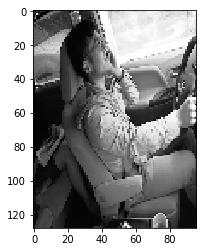
\includegraphics[width=\textwidth]{ae-img1}
        \label{fig:gull}
    \end{subfigure}
    ~ %add desired spacing between images, e. g. ~, \quad, \qquad, \hfill etc. 
      %(or a blank line to force the subfigure onto a new line)
    \begin{subfigure}[b]{0.3\textwidth}
        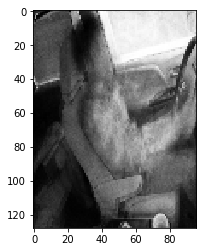
\includegraphics[width=\textwidth]{ae-r1}
        \label{fig:tiger}
    \end{subfigure}
    ~ %add desired spacing between images, e. g. ~, \quad, \qquad, \hfill etc. 
    %(or a blank line to force the subfigure onto a new line)
    \caption{Left one is original image, right is reconstructed. As you see, the hands appear clearly, but phone cannot be seen. It is because phone is small object compared to human and the loss function sees it unimportant.}
  \label{fig:animals}
\end{figure}


\begin{figure}[H]
    \centering
    \begin{subfigure}[b]{0.3\textwidth}
        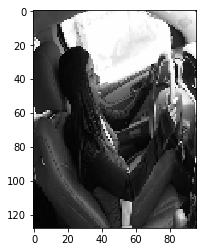
\includegraphics[width=\textwidth]{ae-img2}
        \label{fig:gull}
    \end{subfigure}
    ~ %add desired spacing between images, e. g. ~, \quad, \qquad, \hfill etc. 
      %(or a blank line to force the subfigure onto a new line)
    \begin{subfigure}[b]{0.3\textwidth}
        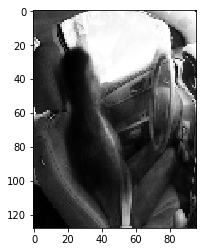
\includegraphics[width=\textwidth]{ae-r2}
        \label{fig:tiger}
    \end{subfigure}
    ~ %add desired spacing between images, e. g. ~, \quad, \qquad, \hfill etc. 
    %(or a blank line to force the subfigure onto a new line)
    \caption{Left one is original image, right is reconstructed. As you see, the hands are very noise as they are black. Autoencoder cannot decide if they are background or not. Also, the background is learned perfectly as it is same in all the images.}
  \label{fig:animals}
\end{figure}
 
\textbf{Regularizer} \\
	In this method, a 5-layered network is used. Third layer is used to reconstruct the image. This gives an affect of regularization. Two objective is optimized jointly. Reconstruction loss function force the classification not to over-fit. The accuracy is again 28 \% and reconstruction loss can be reduced to 0.46. 
\begin{figure}[H]
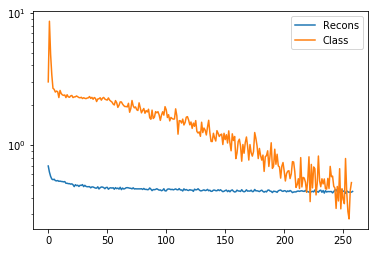
\includegraphics[width=\textwidth]{ae-r}
    \caption{This graph indicates the relation of losses of joint learning. To 0.46, first autoencoder learns features for classification and classification loss decrease meaningfully. But after 0.46, autoencoder stops the learning and classifier become over-fitted. }
\end{figure}
\subsubsection{Variational Autoencoder}
	In auto-encoders, the latent features can be placed in the space without a rule. However, Variational AE forced latent space to obey a distribution. The loss also consist of two parts, one of them reconstruction error and other is KL-divergence that implies the distribution distance from expected one. Also, latent features are sampled from this learned features. This sampling gives a dropout affect.
	In experiment, I use different $\lambda$ values to obtain a good result for reconstruction for
	$$L = L_{reconstruction} + \lambda L_{KL-divergence}$$
For higher $lambda$ first distribution is learned, for lower ones reconstruction is learned. 0.1 is good for reconstruction. However, I cannot obtain a result for classification. Classifier that classifies sampled latent space cannot be optimized. It is because VAE cannot be trained good enough that sampling affects as a very high dropout rate. Even though reconstruction loss less than autoencoder, the sampling make classifier very weak. To sum up, more data or bigger model is needed to overcome this. But, two of them are not ready for this project. If VAE can be trained successfully, it can be used for data generation to expand the dataset artificially.
\begin{figure}[H]
    \centering
    \begin{subfigure}[b]{0.3\textwidth}
        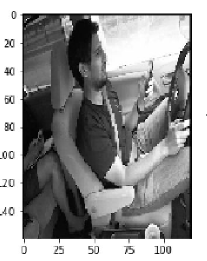
\includegraphics[width=\textwidth]{vae-1.png}
        \label{fig:gull}
    \end{subfigure}
    ~ %add desired spacing between images, e. g. ~, \quad, \qquad, \hfill etc. 
      %(or a blank line to force the subfigure onto a new line)
    \begin{subfigure}[b]{0.3\textwidth}
        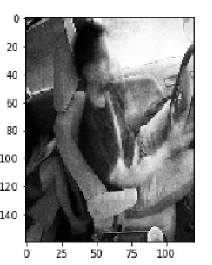
\includegraphics[width=\textwidth]{vae-1r.png}
        \label{fig:tiger}
    \end{subfigure}
    ~ %add desired spacing between images, e. g. ~, \quad, \qquad, \hfill etc. 
    %(or a blank line to force the subfigure onto a new line)
    \caption{Left one is original image, right is reconstructed. As you see, the hands are very clear, and background is nearly perfect.However, the phone is missing. }
  \label{fig:animals}
\end{figure}
\subsection{Imposing Prior}

\subsubsection{CNN}
		CNN is a state of the art model for computer vision tasks as it carries high prior about data. CNN extracts local features and makes abstraction over them. So,a VGG-Net like architecture is used for classification. First layers has big kernels and less filers and last layers have small kernels and more filters.5-layers CNN gives 33\% accuracy with dropout at fully connected layers. CNN can alone increase rate 5\% without any data science or any knowledge.
\subsubsection{Convolutional Autoencoder}
	The reconstruction trick is applied to CNN here. A shallow network tries to reconstruct the image from the last convolution later and a classifier uses this layer as a feature map. This approach increases the accuracy also reconstruction loss is reduced under 0.46. However, the resulting images is not good for human eye. The accuracy is now 38\% which is best result I have. This means that CNN can detect the abstract features but features cannot be interpretable after some layer. Shallow network cannot reconstruct semantically, but it reduces the loss better than others. Also, the phone or coffee can be detected by CNN with an abstract and non-human like manner.
	\begin{figure}[H]
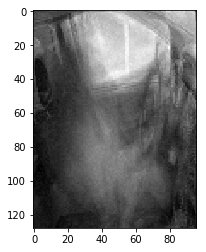
\includegraphics{cae}
    \caption{Reconstruction with plain network cannot be reconstruct the abstract feature of CNN. }
\end{figure}

\section{Conclusion}
	To sum up, In autonomous driving, reasoning is important. Every model has some drawbacks and advantages. Driving is very related with safety of human lives. So, choosing a interpretable model than a high accuracy model is preferred. As known, CNN can very good abstraction but can be faked with some pixel altering. It is because its features cannot be understood after some layers. However, a generative model like autoencoder or variational autoencoder is more informative about its weakness. Also, if there are not sufficient data, auto-encoders enchance the results. Furthermore, variational autoencoder can be used for data-augmentation by generating realistic data.
	There are two missing part in this study. First one is not to use bigger models. It gives more trustable results and provide more practical knowledge. The second one is not to obtain a trained Variational Autoencoder. I used two different loss function, but another solutions could be tested. They are left as future work.

\end{document}
